\documentclass[11pt,a4paper]{article}
\usepackage[utf8]{inputenc}
\usepackage[T1]{fontenc}
\usepackage[spanish,es-noshorthands,es-tabla]{babel}
\usepackage{lmodern}
\usepackage[margin=2.5cm]{geometry}
\usepackage{amsmath,amssymb}
\usepackage{graphicx}
\usepackage{booktabs}
\usepackage{float}
\usepackage{caption}
\usepackage{enumitem}
\usepackage{xurl}
\usepackage[hidelinks]{hyperref}

\captionsetup{font=small,labelfont=bf}
\setlength{\parskip}{0.45em}
\setlength{\parindent}{0pt}
\newcommand{\uno}{\mathbf{1}}
\newcommand{\cut}{\operatorname{cut}}
\newcommand{\vol}{\operatorname{vol}}

\begin{document}

% ------------------------------------------------------------------ PORTADA
\begin{titlepage}
\centering
{\large Universidad Adolfo Ibáñez · Facultad de Ingeniería y Ciencias\par}
{\large Álgebra Lineal y Optimización para Data Science\par}
\vspace{3cm}
{\Huge\bfseries Trabajo Práctico 1\par}
\vspace{0.5cm}
{\LARGE Clustering espectral de países según sus gustos musicales en Spotify\par}
\vspace{2cm}
\begin{tabular}{l}
\toprule
\textbf{Integrantes}\\
\midrule
Max Lastra\\
Benjamín Nuñez\\
\bottomrule
\end{tabular}
\vspace{1.5cm}

\textbf{Base de datos:} \emph{Top Spotify Songs in 73 Countries (Daily Updated)} (Kaggle),\\
Top 50 diario de 72 países, 18-10-2023 a 11-06-2025.
\vfill
{\large Profesores: Martín Ríos-Wilson\par}
{\large Octubre de 2026\par}
\end{titlepage}

\tableofcontents
\newpage

% ------------------------------------------------------------------ INTRODUCCIÓN
\section{Introducción}

En Ciencia de Datos, el clustering busca separar elementos en grupos parecidos por dentro y distintos entre sí. Cuando los datos forman una red, como personas que se comunican o países que escuchan la misma música, esos grupos son comunidades: nodos muy conectados entre sí y poco conectados con el resto. El clustering espectral las encuentra con álgebra lineal: representa la red con las matrices $A$, $D$ y el Laplaciano $L=D-A$, y usa los vectores propios de $L$ de menor valor propio como coordenadas de cada nodo, de forma parecida a como PCA usa vectores propios para resumir datos. En esas coordenadas los grupos quedan separados y $k$-means los encuentra con facilidad.

La relación entre el espectro del Laplaciano y la conectividad de un grafo se estudia desde los años 70, y el método se popularizó a comienzos de los 2000 para segmentar imágenes; hoy también se usa en redes sociales y en biología. Su ventaja es que solo necesita similitudes entre pares de elementos, detecta grupos de formas no convexas y el propio espectro indica cuántas componentes y cuántos grupos hay; su desventaja es que depende de cómo se construye la red, exige elegir el número de grupos y es costoso en redes muy grandes. Representar la red con matrices es útil porque propiedades globales, como sus partes desconectadas o su punto más débil, aparecen en los valores y vectores propios de $L$.

% ------------------------------------------------------------------ DESARROLLO
\section{Desarrollo (Parte I)}

En esta sección, $G=(V,E)$ es un grafo no dirigido y ponderado con $n$ nodos, pesos $a_{ij}=a_{ji}\ge0$ y $a_{ii}=0$. Además, $d_i=\sum_ja_{ij}$, $D=\mathrm{diag}(d_1,\dots,d_n)$ y $L=D-A$.

\subsection{Pregunta 1. Una red como objeto matricial}

(a) $A$ indica qué nodos están conectados y con qué peso. $D$ indica cuánta conexión total tiene cada nodo (su grado). $L=D-A$ combina ambas y, como se ve en la Pregunta 2, mide cuánto cambia una función al recorrer las aristas.

(b) Un vector $x\in\mathbb{R}^n$ se interpreta como la función que asigna el número $x_i$ al nodo $i$. Por ejemplo, $x_i$ puede ser el grado del nodo $i$, o $x_i=1$ si el nodo pertenece a cierto grupo y $0$ si no.

(c) El conjunto $\mathcal{F}(V)=\{f:V\to\mathbb{R}\}$, con suma $(f+g)(v)=f(v)+g(v)$ y producto por escalar $(\alpha f)(v)=\alpha f(v)$, es un espacio vectorial. Las operaciones dan otra función sobre los nodos, y los axiomas se cumplen porque se cumplen en $\mathbb{R}$ evaluando en cada nodo. El neutro es la función nula y el inverso de $f$ es $-f$. Las funciones indicadoras de cada nodo forman una base, así que $\mathcal{F}(V)\cong\mathbb{R}^n$.

\emph{Ejemplo.} Con tres nodos, sean $f=(0{,}5;\ 0{,}8;\ 0)$ y $g=(1;1;0)$ dos funciones sobre ellos. Entonces $f+g=(1{,}5;\ 1{,}8;\ 0)$ y $2f-3g=(-2;\ -1{,}4;\ 0)$.

(d) Si la red es no dirigida, $a_{ij}=a_{ji}$, es decir, $A^\top=A$. Como $D$ es diagonal, $D^\top=D$. Luego $L^\top=D^\top-A^\top=D-A=L$.

\subsection{Pregunta 2. La forma cuadrática del Laplaciano}

Demostración de la identidad. Por un lado, $x^\top Lx=x^\top Dx-x^\top Ax=\sum_{i,j}a_{ij}x_i^2-\sum_{i,j}a_{ij}x_ix_j$, usando que $d_i=\sum_ja_{ij}$. Por otro lado,
\[
\tfrac12\sum_{i,j}a_{ij}(x_i-x_j)^2=\tfrac12\sum_{i,j}a_{ij}x_i^2+\tfrac12\sum_{i,j}a_{ij}x_j^2-\sum_{i,j}a_{ij}x_ix_j .
\]
Por simetría de $A$, las dos primeras sumas son iguales, y juntas valen $\sum_{i,j}a_{ij}x_i^2$. Por lo tanto ambas expresiones coinciden.

(a) Cada término $a_{ij}(x_i-x_j)^2$ es mayor o igual a $0$, luego $x^\top Lx\ge0$ para todo $x$: $L$ es semidefinida positiva.

(b) $x^\top Lx$ suma, sobre todas las aristas, el peso de la arista por el cuadrado de la diferencia entre los valores de sus extremos. Mide la \emph{variación} de la función $x$ sobre la red: es pequeña si $x$ cambia poco entre nodos conectados.

(c) Si los nodos fuertemente conectados (con $a_{ij}$ grande) reciben valores similares, sus términos son casi nulos y $x^\top Lx$ es pequeña. Por eso, las funciones que minimizan $x^\top Lx$ son casi constantes dentro de los grupos densos.

(d) $(L\uno)_i=d_i-\sum_ja_{ij}=0$, luego $L\uno=0$. El vector constante no varía en ninguna arista, así que es un vector propio de valor propio $0$, que es el menor posible porque $L$ es semidefinida positiva. Ese vector no distingue grupos.

\subsection{Pregunta 3. Matriz de incidencia y SVD}

Se orienta cada arista $e=\{i,j\}$ de $i$ a $j$ y se define $B\in\mathbb{R}^{m\times n}$ con $B_{ei}=1$, $B_{ej}=-1$ y $0$ en el resto. Así, $(Bx)_e=x_i-x_j$.

(a) $(B^\top B)_{kl}=\sum_eB_{ek}B_{el}$. Si $k=l$, la suma cuenta las aristas que tocan a $k$, es decir, $d_k$. Si $k\neq l$, solo aporta la arista entre $k$ y $l$ (si existe), con producto $1\cdot(-1)=-1$, es decir, $-a_{kl}$. Luego $B^\top B=D-A=L$.

(b) Con pesos, la fila de cada arista se multiplica por $\sqrt{w_e}$ ($\tilde B=W^{1/2}B$). Repitiendo el cálculo, $\tilde B^\top\tilde B=B^\top WB=L$.

(c) Si $B=U\Sigma V^\top$, entonces $L=B^\top B=V\Sigma^\top U^\top U\Sigma V^\top=V\Sigma^\top\Sigma V^\top$, porque $U^\top U=I$.

(d) $\Sigma^\top\Sigma$ es diagonal con entradas $\sigma_i^2$, así que $L=V(\Sigma^\top\Sigma)V^\top$ es una diagonalización ortogonal de $L$. Por lo tanto, los valores propios de $L$ son los cuadrados de los valores singulares de $B$ ($\lambda_i=\sigma_i^2$), y los vectores propios de $L$ son los vectores singulares derechos de $B$ (columnas de $V$).

\subsection{Pregunta 4. El espectro y la conectividad}

(a) $L$ es real y simétrica. Por el teorema espectral, $L=Q\Lambda Q^\top$ con $Q$ ortogonal, y las columnas de $Q$ forman una base ortonormal de $\mathbb{R}^n$ de vectores propios de $L$.

(b) Sean $C_1,\dots,C_k$ las componentes conexas y $\uno_{C_r}$ sus vectores indicadores. Si $i\in C_r$, entonces $(L\uno_{C_r})_i=d_i-\sum_{j\in C_r}a_{ij}=0$, porque todos los vecinos de $i$ están en $C_r$. Si $i\notin C_r$, entonces $(L\uno_{C_r})_i=-\sum_{j\in C_r}a_{ij}=0$, porque no hay aristas entre componentes. Luego los $k$ vectores $\uno_{C_r}$ están en $\ker L$. Como tienen soportes disjuntos, son linealmente independientes.

(c) Si $Lx=0$, entonces $x^\top Lx=0$, y por la Pregunta 2, $x_i=x_j$ en cada arista. Así $x$ es constante en cada componente, es decir, $x\in\mathrm{span}\{\uno_{C_r}\}$. Por lo tanto, la multiplicidad del valor propio 0 es igual al número de componentes conexas.

(d) Si $\lambda_2=0$, la red está desconectada. Si $\lambda_2$ es positivo pero pequeño, es conexa pero se puede separar cortando pocas aristas o aristas débiles. Si $\lambda_2$ es relativamente grande, la red está bien conectada y no tiene un corte barato.

(e) El vector de Fiedler minimiza $x^\top Lx$ entre los vectores unitarios ortogonales a $\uno$ (Pregunta 5f). Al ser ortogonal a $\uno$, debe tener coordenadas positivas y negativas. Al minimizar la variación, asigna valores parecidos a nodos muy conectados. Por eso cambia de signo justamente donde hay pocas conexiones, y su signo sugiere una separación de la red.

\subsection{Pregunta 5. Partición como problema de optimización}

(a) Una partición $V=S\cup\bar S$ se representa con $s\in\{-1,1\}^n$, donde $s_i=1$ si $i\in S$ y $s_i=-1$ si $i\in\bar S$.

(b) $\cut(S,\bar S)=\sum_{i\in S,j\in\bar S}a_{ij}$. Como $(s_i-s_j)^2$ vale $4$ si $i$ y $j$ están en grupos distintos y $0$ si no, se tiene $\cut(S,\bar S)=\tfrac14s^\top Ls$.

(c) El corte no considera el tamaño de los grupos. Separar un solo nodo de grado bajo cuesta muy poco, por lo que el mínimo tiende a aislar nodos periféricos.

(d) Los criterios balanceados dividen el corte por el tamaño de cada grupo:
\[
\mathrm{RatioCut}=\frac{\cut(S,\bar S)}{|S|}+\frac{\cut(S,\bar S)}{|\bar S|},\qquad
\mathrm{NCut}=\frac{\cut(S,\bar S)}{\vol(S)}+\frac{\cut(S,\bar S)}{\vol(\bar S)},\qquad \vol(S)=\sum_{i\in S}d_i .
\]
Ambos se hacen grandes si un grupo es muy pequeño. RatioCut equilibra el número de nodos y NCut equilibra la suma de grados.

(e) Para RatioCut se define $f_i=\sqrt{|\bar S|/|S|}$ si $i\in S$ y $f_i=-\sqrt{|S|/|\bar S|}$ si $i\in\bar S$. Se verifica que $f^\top Lf=n\cdot\mathrm{RatioCut}(S,\bar S)$, que $\sum_if_i=0$ y que $\|f\|^2=n$. Minimizar RatioCut equivale entonces a minimizar $f^\top Lf$ sobre esos vectores discretos. La relajación permite que $f$ sea cualquier vector de $\mathbb{R}^n$ con $f\perp\uno$ y $\|f\|=\sqrt n$, y así se obtiene la minimización de una forma cuadrática del Laplaciano. Con NCut se llega de la misma forma al Laplaciano normalizado $L_{sym}=I-D^{-1/2}AD^{-1/2}$.

(f) Sea $q_1=\uno/\sqrt n,q_2,\dots,q_n$ una base ortonormal de vectores propios con $0=\lambda_1\le\lambda_2\le\dots$. Si $x=\sum_ic_iq_i$, las restricciones dan $c_1=0$ y $\sum_ic_i^2=1$. Luego
\[
x^\top Lx=\sum_{i\ge2}\lambda_ic_i^2\ \ge\ \lambda_2\sum_{i\ge2}c_i^2=\lambda_2,
\]
y la igualdad se alcanza con $x=q_2$. La solución es el vector propio del segundo menor valor propio.

(g) Para obtener una partición a partir de la solución continua $v_2$, se asigna cada nodo según el signo de su coordenada: $S=\{i:v_2(i)\ge0\}$. Otra opción es ordenar los nodos por $v_2$ y elegir el umbral que minimiza NCut.

\subsection{Pregunta 6. Clustering espectral con $k$ grupos}

Sea $U=[v_1\cdots v_k]$ la matriz con los $k$ vectores propios de menor valor propio.

(a--b) La fila $i$ de $U$ contiene los valores de las $k$ funciones más suaves de la red en el nodo $i$. Así, cada nodo queda representado como un punto de $\mathbb{R}^k$. Si la red tuviera $k$ componentes, todos los nodos de una misma componente caerían en el mismo punto.

(c) En esta representación, los nodos muy conectados entre sí quedan cerca, porque los vectores propios varían poco entre ellos. La distancia euclidiana entre filas mide entonces qué tan probable es que dos nodos estén en la misma comunidad.

(d) Se aplica $k$-means a las filas de $U$ y cada nodo se asigna al grupo de su fila. Con $L_{sym}$, antes se normaliza cada fila a norma 1.

(e) Las características originales tienen dimensión muy alta y no usan la estructura de red. Las filas de $A$ solo contienen información local, es decir, los vecinos directos. La representación espectral tiene dimensión $k$ y resume la estructura global de la red, por lo que los grupos quedan compactos y separados.

(f) Si hay $k$ grupos bien separados, $\lambda_1,\dots,\lambda_k$ son casi $0$ y $\lambda_{k+1}$ es claramente mayor. Por eso se elige el $k$ con el mayor salto $\lambda_{k+1}-\lambda_k$ (\emph{eigengap}).

(g) Dos situaciones problemáticas:
\begin{itemize}[leftmargin=1.5em]
\item Con grados muy distintos, el Laplaciano no normalizado separa nodos sueltos de grado bajo.
\item Si no hay un salto claro en los valores propios, la elección de $k$ es ambigua, y si dos valores propios son casi iguales, los vectores propios (y la partición) se vuelven inestables.
\end{itemize}

% ------------------------------------------------------------------ APLICACIÓN
\section{Aplicación}

\subsection{Problema y datos}

Fuente. \emph{Top Spotify Songs in 73 Countries (Daily Updated)}, publicado en Kaggle con licencia ODC-By. Contiene el Top 50 diario de Spotify de cada país. Se usó todo el período disponible: del 18-10-2023 al 11-06-2025, es decir, 583 días y 2.110.316 filas. El notebook descarga los datos automáticamente.

La red.
\begin{itemize}[leftmargin=1.5em]
\item Nodos: los 72 países con ranking propio. Se excluye el Top 50 Global, que no es un país.
\item Aristas: unen cada país con sus 12 países de gustos más parecidos.
\item Pesos: la similitud coseno entre sus perfiles musicales.
\item Dirección: la red es no dirigida y tiene 665 aristas.
\end{itemize}

Pregunta de análisis. \emph{¿Cómo se agrupan los países según lo que escuchan en Spotify, y qué explica mejor esos grupos: el idioma, la geografía o el clima? ¿Qué rol cumplen los éxitos globales?} Subpreguntas:
\begin{enumerate}[leftmargin=1.5em]
\item ¿Cuántos grupos sugiere el espectro?
\item ¿Las comunidades coinciden más con idioma, continente o clima?
\item ¿Qué cambia al quitar los éxitos globales?
\item ¿Con quién se agrupa Chile y qué países son puente?
\end{enumerate}

Por qué clustering espectral. No sabemos de antemano cuántos grupos hay y solo tenemos similitudes entre países. El espectro indica directamente si la red se separa en bloques, cuántos grupos hay y qué países están en la frontera.

\subsection{Construcción y preparación de la red}\label{sec:construccion}

Decisiones de preprocesamiento.
\begin{itemize}[leftmargin=1.5em]
\item Se excluyó el Top 50 Global.
\item Se conservaron las posiciones $\le50$ y se eliminaron 90 filas duplicadas.
\item Cada canción se identificó por \emph{nombre + artistas}, porque una misma canción puede tener varios identificadores según el mercado. Así quedan 23.021 canciones, contra 24.977 identificadores.
\end{itemize}

Perfiles y similitud. Cada país $c$ se representa con el vector $x_c$, donde $x_c(s)$ es el número de días que la canción $s$ estuvo en su Top 50. La similitud entre dos países es el coseno $s_{ij}=\langle x_i,x_j\rangle/(\|x_i\|\|x_j\|)$. El coseno compara proporciones, así que no importa que algunos países tengan menos días de datos (Reino Unido tiene 418).

Construcción de la red. Casi todos los países comparten algún éxito global, así que conectar a todos con todos diluye la estructura. Se conectó cada país con sus $k$ más parecidos y se simetrizó la red. Esto garantiza que no haya nodos aislados y que no haya \emph{loops}.

Elección de $k$ y componentes conexas. Se eligió el menor $k$ que deja la red conexa, que resultó ser $k=12$. Para $k\le11$ la red tiene dos componentes: los 17 países hispanohablantes de América Latina más España, y el resto del mundo (Figura~\ref{fig:conect}). Es decir, ningún país hispano tiene a un país no hispano entre sus 11 más parecidos. En ese caso el valor propio $0$ es doble, como predice la Pregunta 4c.

\begin{figure}[H]
\centering
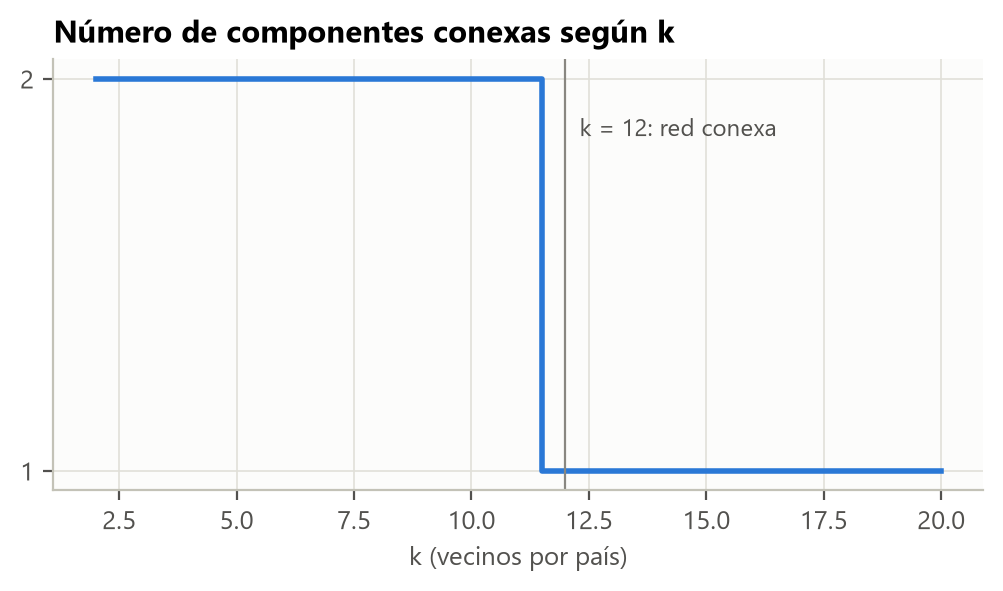
\includegraphics[width=0.6\textwidth]{figuras/fig01_conectividad.png}
\caption{Número de componentes conexas según el número de vecinos $k$.}\label{fig:conect}
\end{figure}

Atributos para evaluar. Para cada país se registró su continente, su idioma principal y su clima. El clima se definió según dónde vive la población: a cada ciudad de más de 15.000 habitantes (GeoNames) se le asignó su clase climática Köppen-Geiger 1991--2020 y su temperatura media (WorldClim), y se calculó la proporción de población urbana en cada grupo (Tropical, Seco, Templado, Continental o Polar). Un país es ``Variado'' solo si es imposible encasillarlo: ningún grupo reúne al menos el 60\,\% de la población y la temperatura varía en $\pm3\,^\circ$C o más entre sus ciudades. Así, EE.UU. (53\,\% templado, $\pm4{,}6\,^\circ$C) queda Variado y Brasil (63\,\% tropical) queda Tropical. Los países variados son EE.UU., México, Bolivia, Ecuador y Guatemala.

\subsection{Implementación del método espectral}

El notebook \texttt{clustering\_espectral\_spotify.ipynb} implementa con \texttt{numpy}:
\begin{enumerate}[leftmargin=1.5em]
\item la construcción de $A$, $D=\mathrm{diag}(A\uno)$, $L=D-A$ y $L_{sym}=I-D^{-1/2}AD^{-1/2}$;
\item el cálculo de valores y vectores propios con \texttt{numpy.linalg.eigh};
\item la representación espectral: los $k$ primeros vectores propios de $L_{sym}$, con cada fila normalizada a norma 1;
\item $k$-means de \texttt{scikit-learn} (50 inicializaciones, semilla fija).
\end{enumerate}
Se usa $L_{sym}$ porque los grados son muy heterogéneos: van de $0{,}07$ (Nigeria) a $15{,}2$ (Suiza).

\subsection{Resultados e interpretación}

Espectro y \emph{eigengap}. Los primeros valores propios de $L_{sym}$ son $0$; $0{,}0003$; $0{,}313$; $0{,}384$; $0{,}661$; \dots{} El mayor salto ocurre después de $\lambda_2$ y el segundo después de $\lambda_4$ (Figura~\ref{fig:espectro}). Por eso se analizan $k=2$ y $k=4$. Además, $\lambda_2\approx0$: la red es conexa, pero está casi separada en dos bloques.

\begin{figure}[H]
\centering
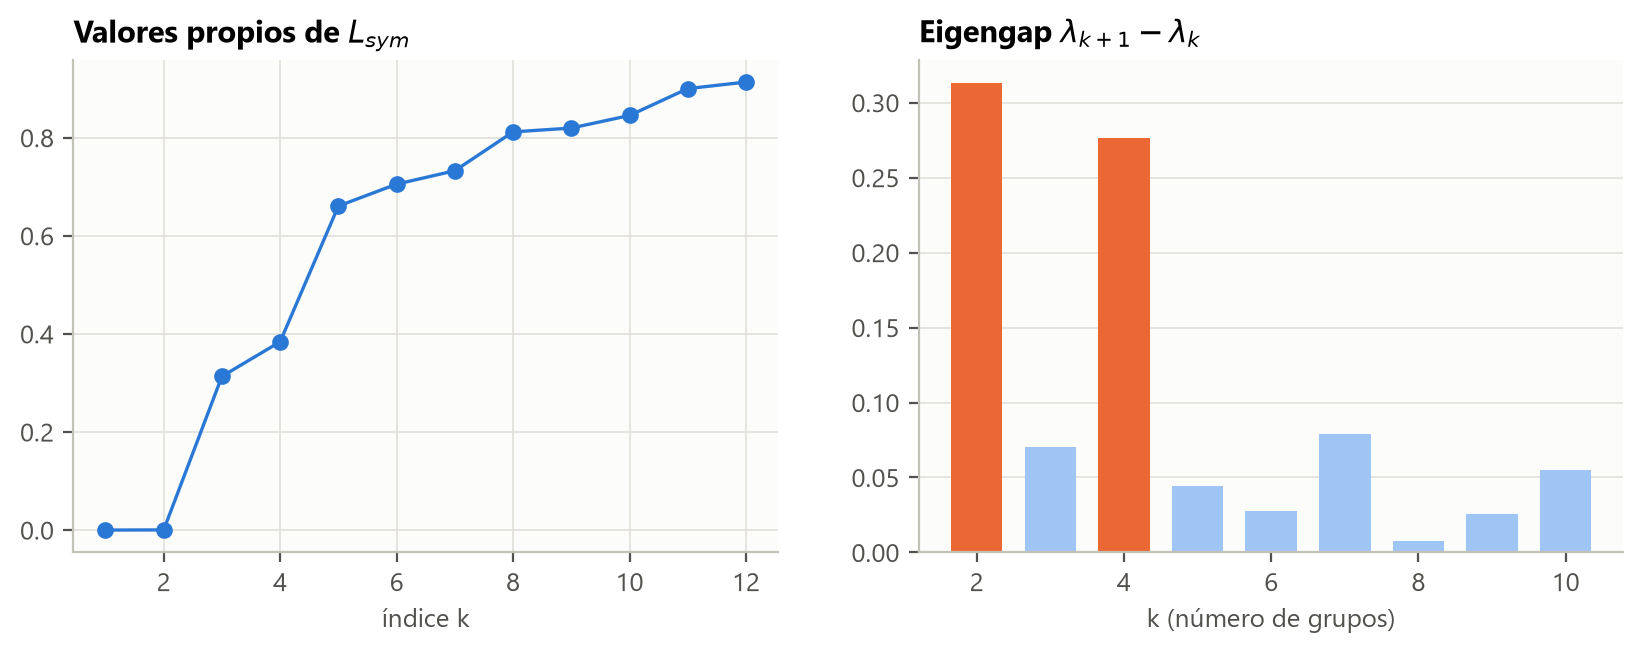
\includegraphics[width=0.9\textwidth]{figuras/fig02_espectro_eigengap.png}
\caption{Valores propios de $L_{sym}$ y \emph{eigengap}. Los saltos más grandes ocurren tras $k=2$ y tras $k=4$.}\label{fig:espectro}
\end{figure}

Vector de Fiedler. Su signo separa exactamente a los 18 países hispanos del resto (Figura~\ref{fig:fiedler}). Como $\lambda_2$ es casi cero, el vector es prácticamente constante dentro de cada bloque.

\begin{figure}[H]
\centering
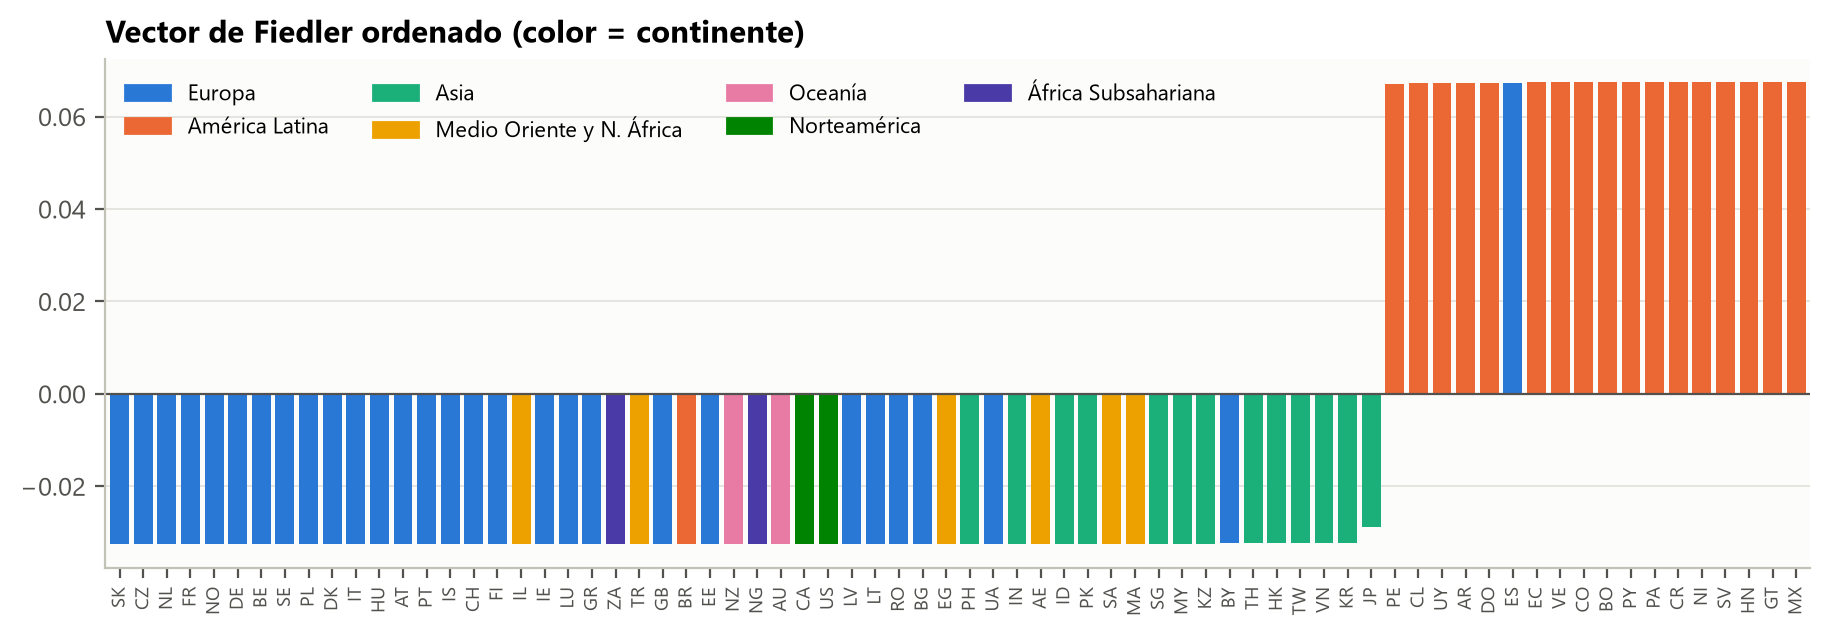
\includegraphics[width=\textwidth]{figuras/fig03_fiedler.png}
\caption{Vector de Fiedler ordenado, coloreado por continente.}\label{fig:fiedler}
\end{figure}

Comunidades. Con $k=2$ se obtienen el bloque hispano (18 países) y el resto del mundo (54). Con $k=4$ (Figura~\ref{fig:mapa}):
\begin{itemize}[leftmargin=1.5em]
\item Hispano (18): América Latina hispanohablante y España.
\item Europa y mundo anglosajón (33): Europa occidental, nórdica, central y báltica, EE.UU., Canadá, Australia, Nueva Zelanda, Sudáfrica, Nigeria, Israel, Turquía y Brasil.
\item Asia, Medio Oriente y Europa del Este (19).
\item Sur de Asia (2): India y Pakistán.
\end{itemize}
La Figura~\ref{fig:emb} muestra la representación espectral: los 18 países hispanos caen prácticamente en un mismo punto.

\begin{figure}[H]
\centering
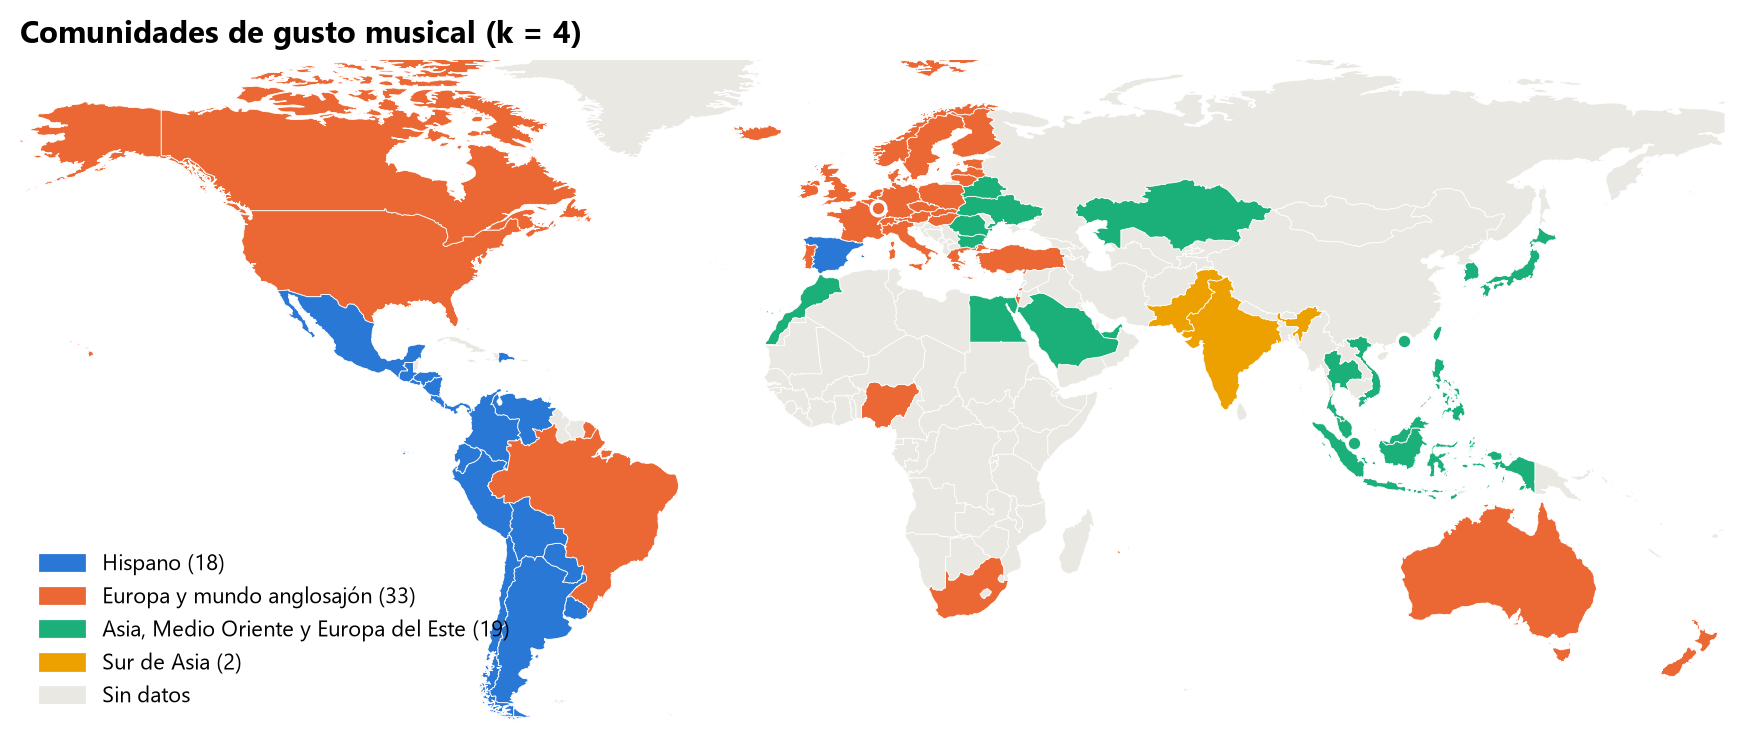
\includegraphics[width=\textwidth]{figuras/fig04_mapa_k4.png}
\caption{Comunidades obtenidas con clustering espectral ($k=4$).}\label{fig:mapa}
\end{figure}

\begin{figure}[H]
\centering
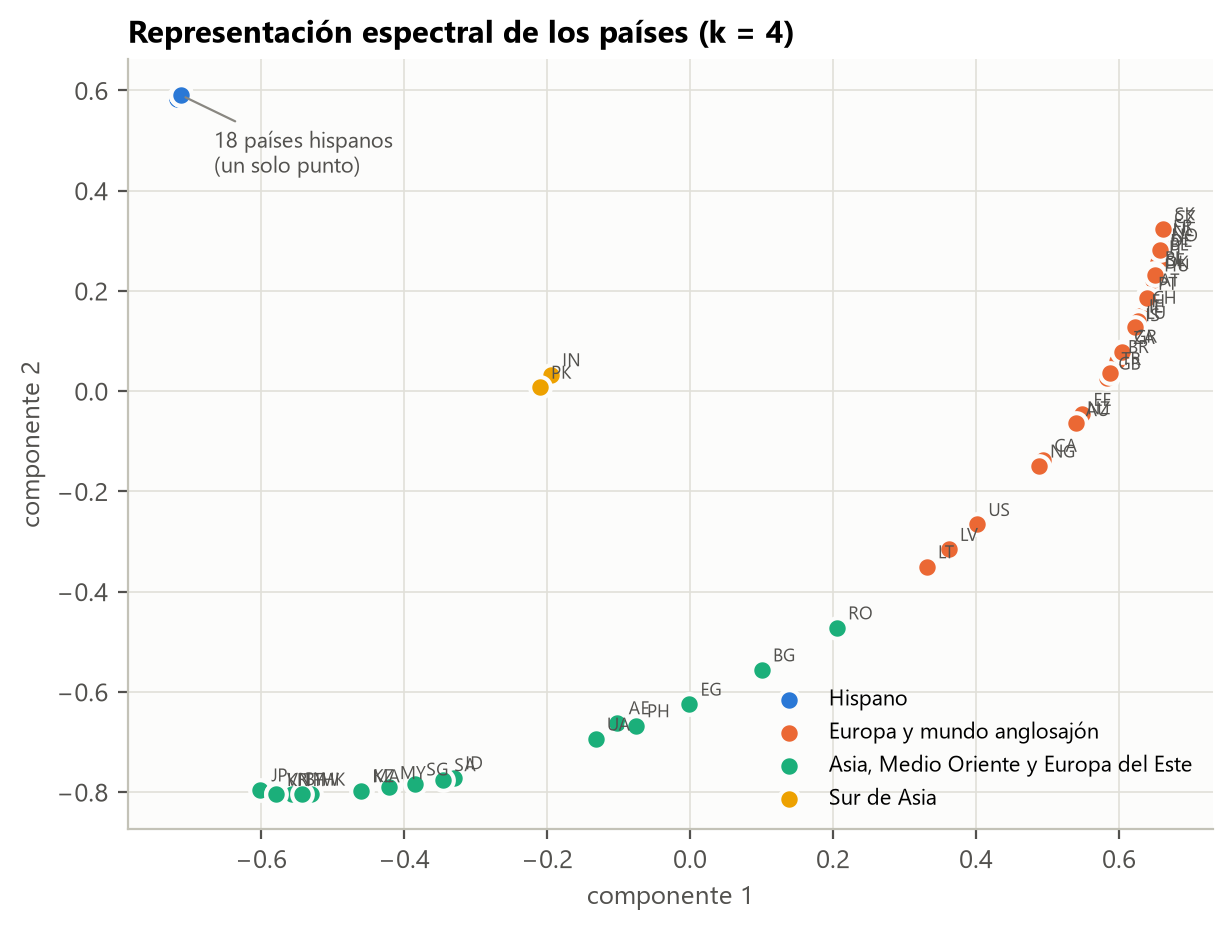
\includegraphics[width=0.62\textwidth]{figuras/fig05_representacion_espectral.png}
\caption{Representación espectral de los países ($k=4$), proyectada a dos dimensiones.}\label{fig:emb}
\end{figure}

En la red (Figura~\ref{fig:red}), la única arista entre el bloque hispano y el resto es Japón–Perú, con similitud $0{,}034$. Se explica casi por completo por canciones de K-pop que estuvieron muchos días en el Top 50 de ambos países, como \emph{Who} de Jimin y \emph{Seven} de Jung Kook.

\begin{figure}[H]
\centering
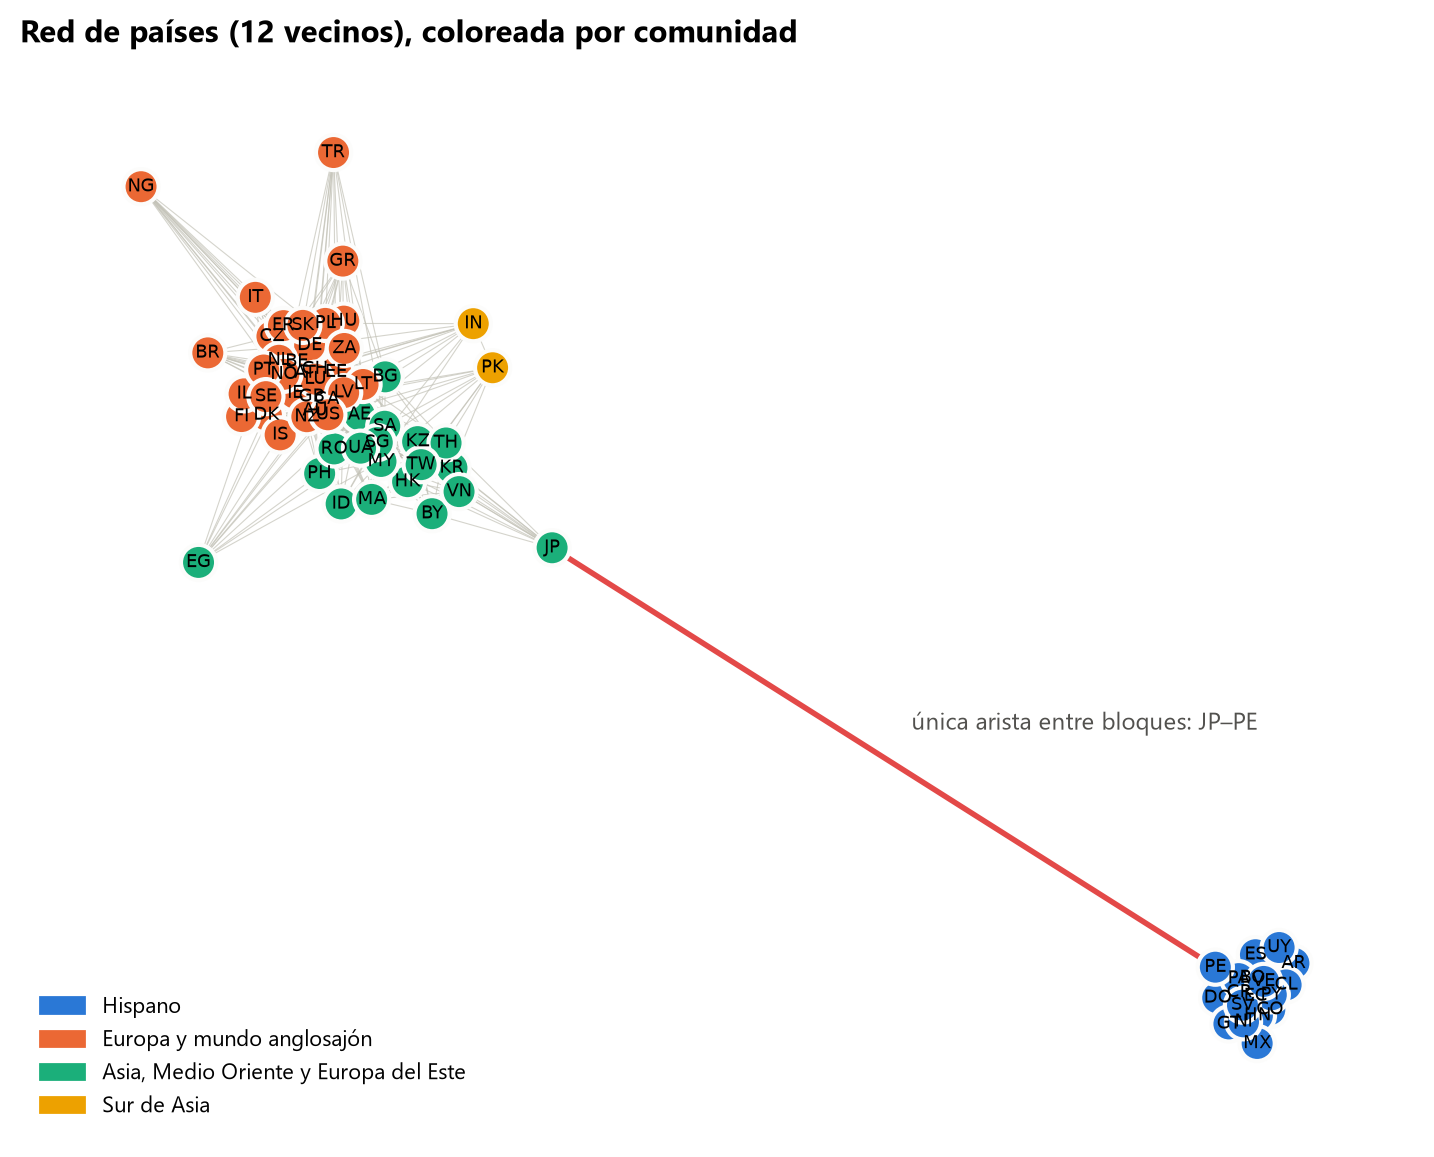
\includegraphics[width=0.8\textwidth]{figuras/fig06_red.png}
\caption{Red de países (12 vecinos), coloreada por comunidad. La arista destacada es la única entre bloques.}\label{fig:red}
\end{figure}

¿Idioma, geografía o clima? Se compararon las comunidades con cada atributo mediante el AMI (información mutua ajustada), que vale $0$ para una partición al azar y $1$ para una coincidencia perfecta (Tabla~\ref{tab:eval}). El continente es el atributo que más coincide, seguido por el idioma, y el clima es el que menos explica. Igualmente, el idioma explica casos que la geografía no explica: España se agrupa con América Latina y no con Europa, y Brasil no se agrupa con sus vecinos hispanohablantes.

El AMI se calcula a partir de la información mutua entre la partición en comunidades $U$ y la categoría $V$:
\[
\mathrm{AMI}(U,V)=\frac{\mathrm{MI}(U,V)-E[\mathrm{MI}]}{\tfrac{1}{2}\big(H(U)+H(V)\big)-E[\mathrm{MI}]},
\]
\[
\mathrm{MI}(U,V)=\sum_{i,j}\frac{n_{ij}}{n}\log\frac{n\,n_{ij}}{a_i\,b_j},\qquad
H(U)=-\sum_i\frac{a_i}{n}\log\frac{a_i}{n},
\]
donde $n$ es el número de países, $n_{ij}$ el número de países que están en la comunidad $i$ y en la categoría $j$, $a_i$ y $b_j$ los tamaños de la comunidad y de la categoría, y $E[\mathrm{MI}]$ la información mutua esperada si los países se repartieran al azar entre grupos de los mismos tamaños. Restar $E[\mathrm{MI}]$ permite comparar atributos con distinto número de categorías, como el continente (7) y el idioma (más de 30).

\begin{table}[H]
\centering\small
\caption{AMI de las comunidades con cada atributo y modularidad de la partición.}\label{tab:eval}
\begin{tabular}{lcc}
\toprule
 & $\mathbf{k=2}$ & $\mathbf{k=4}$\\
\midrule
AMI continente & 0,401 & 0,514\\
AMI idioma & 0,169 & 0,313\\
AMI clima & 0,131 & 0,189\\
Modularidad & 0,439 & 0,485\\
Tamaños & 18 / 54 & 18 / 33 / 19 / 2\\
\bottomrule
\end{tabular}
\end{table}

Chile y países puente. Chile está en el bloque hispano, y su país más parecido es Perú ($0{,}574$), seguido de Bolivia ($0{,}534$), Paraguay ($0{,}529$) y Ecuador ($0{,}513$). Para medir qué países son puente se usó el \emph{índice de frontera}, la fracción del peso de las aristas de un país que va hacia otras comunidades. El de Chile es $0$: todos sus vecinos son hispanos, de modo que Chile está en el centro de su bloque. Los países puente son Rumania ($0{,}66$), Bulgaria ($0{,}66$), Ucrania ($0{,}61$), Emiratos ($0{,}60$) y Egipto ($0{,}55$), que reparten su afinidad entre Europa y Asia/Medio Oriente.

\subsection{Diseño experimental}

Experimento 1: Laplaciano no normalizado frente a normalizado (Tabla~\ref{tab:e1}). Con $k=2$ ambos dan la misma partición. Con $k=4$, el Laplaciano no normalizado forma dos grupos de un solo país (Nigeria y Turquía), que son nodos de grado bajo cuyo corte es barato, tal como se explicó en la Pregunta 5c. En la Figura~\ref{fig:lnorm} se ve que su segundo vector propio también separa al bloque hispano. El normalizado entrega grupos interpretables y con mayor modularidad.

\begin{table}[H]
\centering\small
\caption{Experimento 1: comparación de Laplacianos con $k=4$.}\label{tab:e1}
\setlength{\tabcolsep}{4pt}
\begin{tabular}{lccccc}
\toprule
\textbf{Laplaciano} & \textbf{Tamaños} & \textbf{AMI cont.} & \textbf{AMI idioma} & \textbf{Modul.} & \textbf{Grupos de 1}\\
\midrule
$L$ (no normalizado) & 52 / 1 / 18 / 1 & 0,428 & 0,171 & 0,439 & Nigeria, Turquía\\
$L_{sym}$ (normalizado) & 33 / 18 / 19 / 2 & 0,514 & 0,313 & 0,485 & ---\\
\bottomrule
\end{tabular}
\end{table}

\begin{figure}[H]
\centering
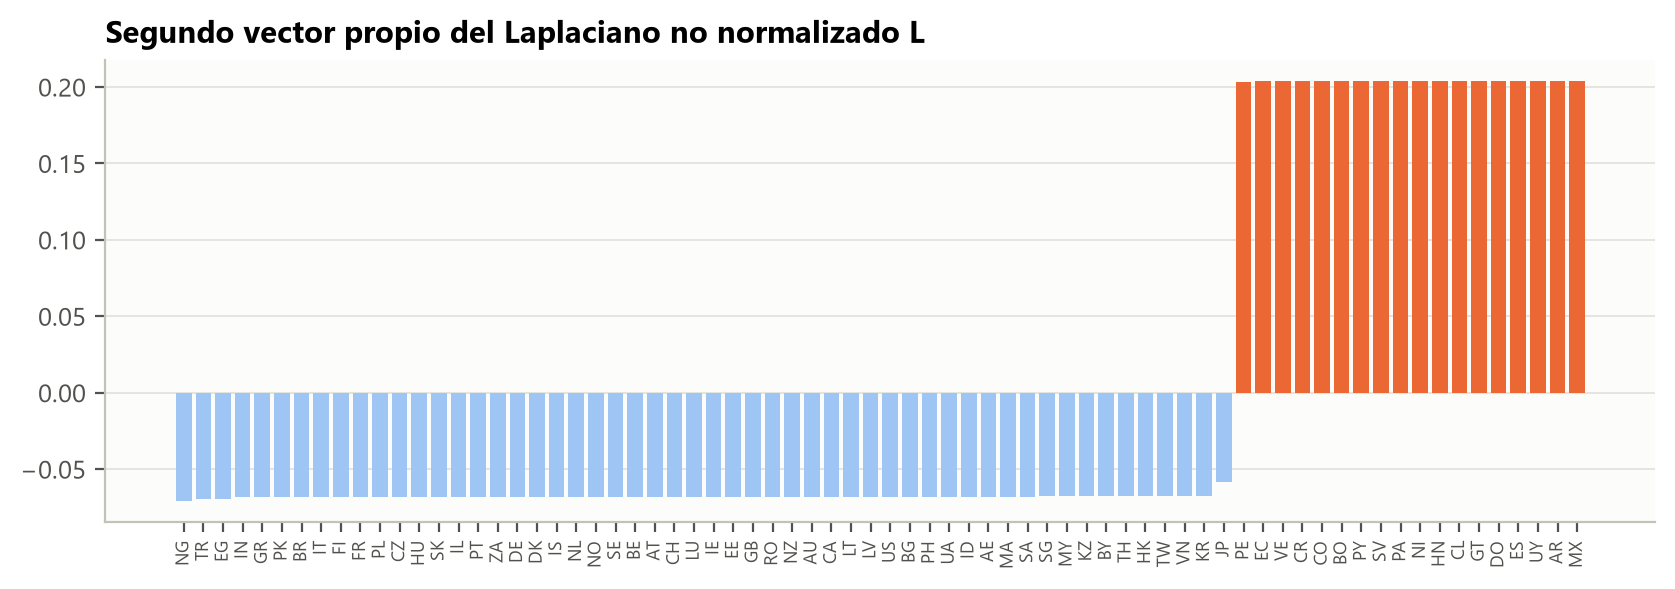
\includegraphics[width=0.85\textwidth]{figuras/fig07_laplaciano_no_normalizado.png}
\caption{Segundo vector propio del Laplaciano no normalizado.}\label{fig:lnorm}
\end{figure}

Experimento 2: quitar los éxitos globales (Tabla~\ref{tab:e2}). Se eliminaron las 313 canciones que estuvieron en el Top 50 de al menos el 30\,\% de los países, como \emph{Die With A Smile}, presente en el 95,8\,\% de ellos. Luego se repitió todo el procedimiento. La similitud mediana entre países cae de $0{,}056$ a casi $0$: los éxitos globales sostienen casi toda la similitud. El bloque hispano se mantiene, pero ahora el \emph{eigengap} sugiere 7 grupos (Figura~\ref{fig:local}):
\begin{itemize}[leftmargin=1.5em]
\item Brasil y Portugal forman un bloque lusófono.
\item Italia se une al bloque hispano.
\item Emiratos Árabes se une a India y Pakistán.
\item Marruecos queda con Europa continental.
\end{itemize}
En esta red el idioma explica bastante más (AMI de $0{,}31$ a $0{,}45$). Los éxitos globales esconden diferencias locales que se relacionan sobre todo con el idioma.

\begin{table}[H]
\centering\small
\caption{Experimento 2: con y sin los éxitos globales.}\label{tab:e2}
\begin{tabular}{lcc}
\toprule
 & \textbf{Todas las canciones ($k=4$)} & \textbf{Sin éxitos globales ($k=7$)}\\
\midrule
AMI continente & 0,514 & 0,511\\
AMI idioma & 0,313 & 0,450\\
AMI clima & 0,189 & 0,204\\
Modularidad & 0,485 & 0,474\\
\bottomrule
\end{tabular}
\end{table}

\begin{figure}[H]
\centering
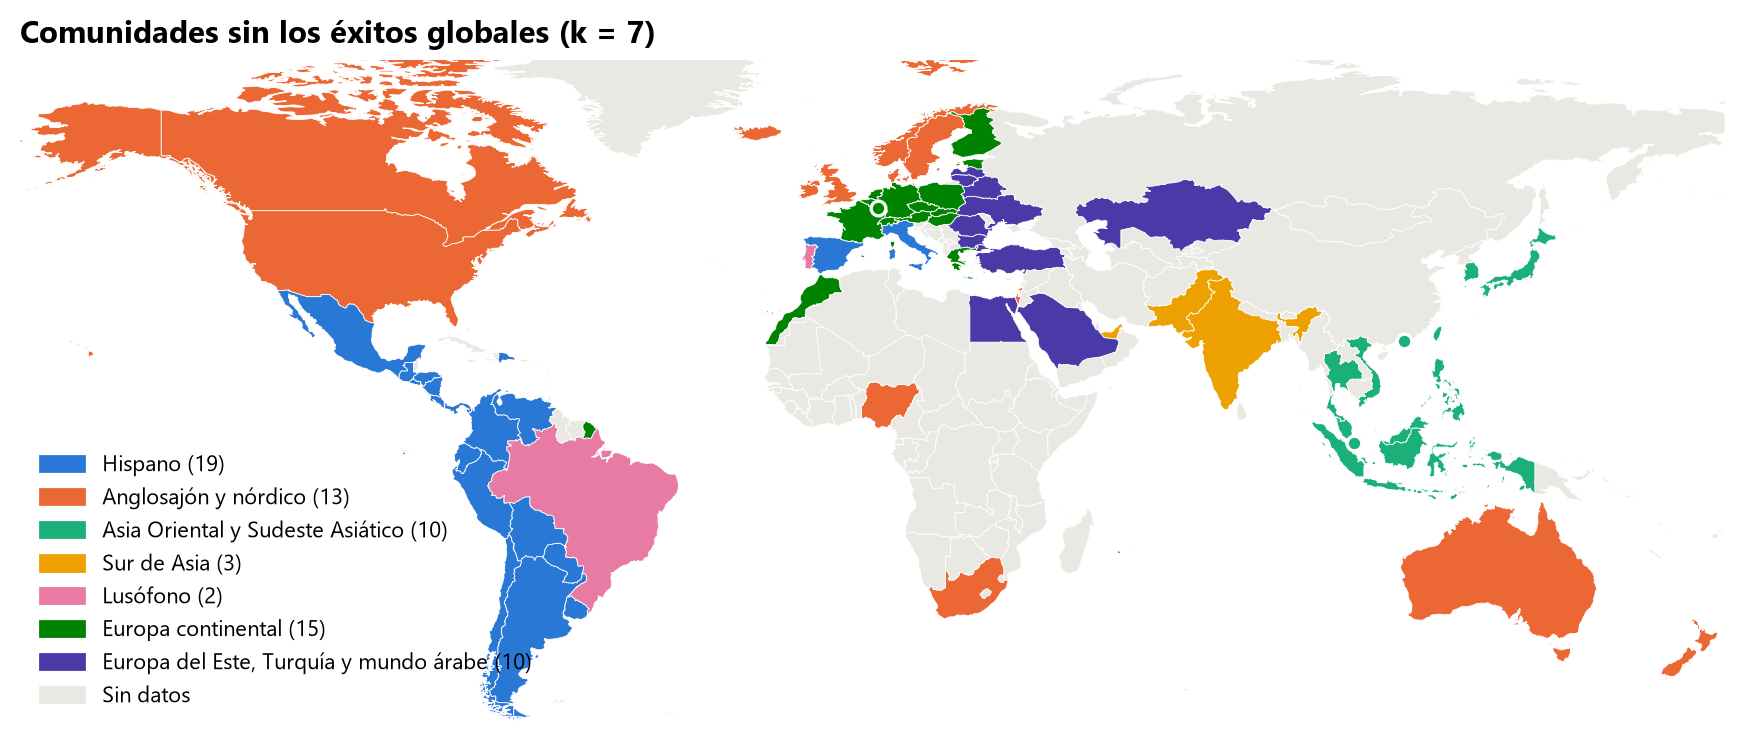
\includegraphics[width=\textwidth]{figuras/fig08_mapa_sin_globales.png}
\caption{Comunidades al quitar los éxitos globales ($k=7$, elegido por \emph{eigengap}).}\label{fig:local}
\end{figure}

Experimento 3: red con pesos frente a red sin pesos (Tabla~\ref{tab:e3}). Se mantuvieron exactamente las mismas aristas, porque cada país sigue conectado con sus 12 países más parecidos, pero todas pasaron a valer 1. Con $k=2$ la partición es idéntica, de modo que el bloque hispano no depende de los pesos. Sin pesos, $\lambda_2$ sube de $0{,}0003$ a $0{,}004$, porque la arista débil Japón–Perú vale lo mismo que cualquier otra, y el \emph{eigengap} deja de apoyar $k=4$ (Figura~\ref{fig:pesos}a). Con $k=4$ la partición cambia bastante (ARI $=0{,}55$ con la partición base, donde 1 indica particiones idénticas): el mundo anglosajón se separa de Europa continental y desaparece el grupo India–Pakistán, ya que India queda con Europa continental, lo que no tiene sentido musical (Figura~\ref{fig:pesos}b). La modularidad baja de $0{,}49$ a $0{,}44$. Los pesos importan para la estructura más fina, porque evitan que las conexiones débiles cuenten igual que las fuertes.

\begin{table}[H]
\centering\small
\caption{Experimento 3: red con pesos y sin pesos.}\label{tab:e3}
\begin{tabular}{lcc}
\toprule
 & \textbf{Con pesos (base)} & \textbf{Sin pesos}\\
\midrule
$\lambda_2$ & 0,0003 & 0,004\\
$k$ sugerido por el \emph{eigengap} & 2 y 4 & 2 y 3\\
Tamaños ($k=4$) & 18 / 33 / 19 / 2 & 18 / 25 / 15 / 14\\
AMI continente & 0,514 & 0,503\\
AMI idioma & 0,313 & 0,356\\
AMI clima & 0,189 & 0,150\\
Modularidad & 0,485 & 0,436\\
\bottomrule
\end{tabular}
\end{table}

\begin{figure}[H]
\centering
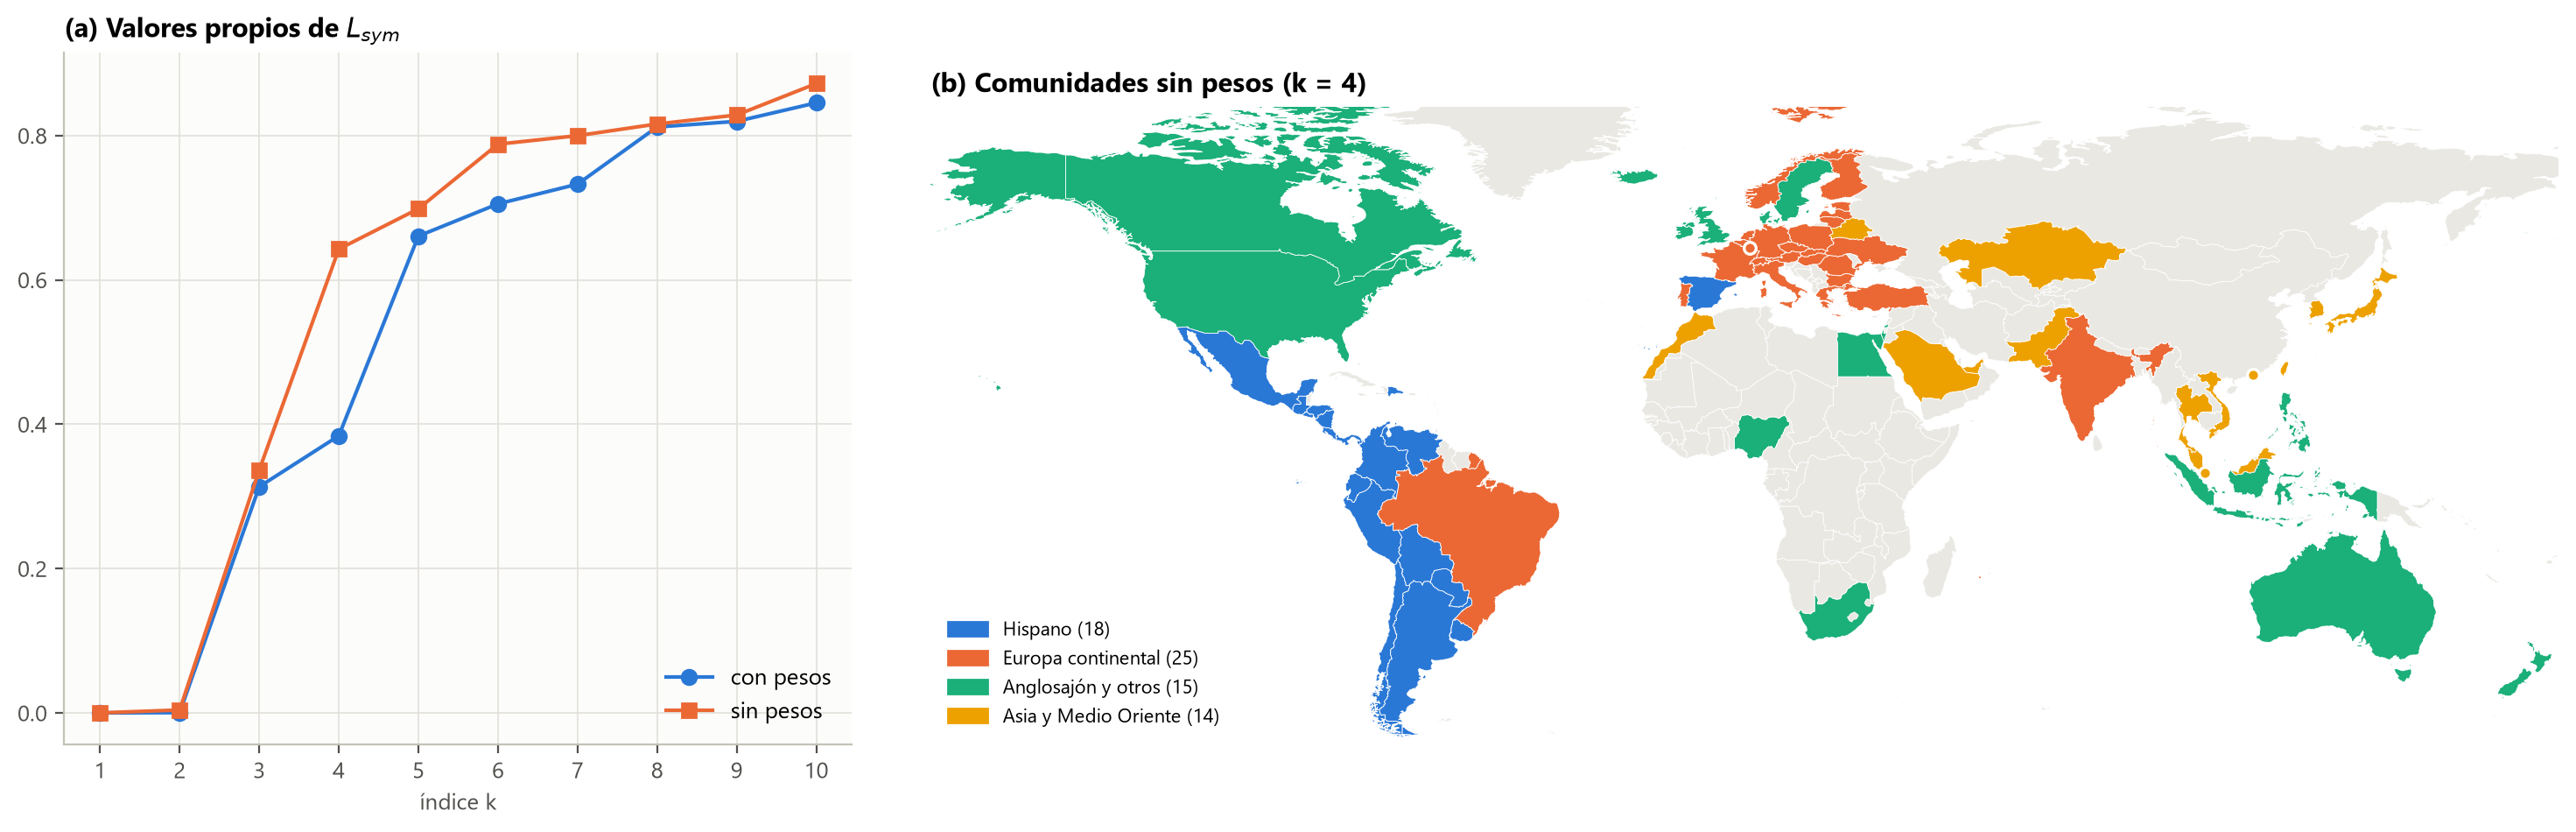
\includegraphics[width=\textwidth]{figuras/fig09_sin_pesos.png}
\caption{(a) Valores propios de $L_{sym}$ con y sin pesos. (b) Comunidades de la red sin pesos ($k=4$).}\label{fig:pesos}
\end{figure}

\subsection{Limitaciones y extensiones}

Limitaciones.
\begin{itemize}[leftmargin=1.5em]
\item Solo se observa el Top 50 de cada país.
\item Spotify no opera en algunos mercados grandes, como China.
\item Algunos países tienen días sin datos.
\item La regla de 12 vecinos obliga a conectar a países de gusto muy local con vecinos poco parecidos (por ejemplo, Japón–Perú).
\item El idioma principal es discutible en países multilingües.
\item La clasificación climática es sensible en casos límite, como Chile, que queda empatado entre seco y templado.
\item El grupo India–Pakistán tiene solo dos países.
\end{itemize}

Extensión propuesta. Construir una red por mes (red temporal) para estudiar si las comunidades cambian a lo largo del año, por ejemplo con los éxitos de verano de cada hemisferio. También se podrían comparar los resultados con métodos que maximizan la modularidad, como Louvain.

% ------------------------------------------------------------------ CONCLUSIONES
\section{Conclusiones}

\begin{enumerate}[leftmargin=1.5em]
\item El espectro muestra dos grandes bloques de gusto musical: el hispano (América Latina hispanohablante y España) y el resto del mundo. Para menos de 12 vecinos aparece como dos componentes conexas (valor propio $0$ doble), y con 12 vecinos como un $\lambda_2$ casi nulo. Con $k=4$ se separan además Europa y el mundo anglosajón; Asia, Medio Oriente y Europa del Este; y el sur de Asia.
\item El continente es lo que más coincide con las comunidades, seguido por el idioma, y el clima es lo que menos las explica. El idioma explica casos que la geografía no explica: España con América Latina y Brasil aparte.
\item Los éxitos globales sostienen casi toda la similitud entre países. Al quitarlos aparece una estructura más local y ligada al idioma (bloque lusófono, Italia con el bloque hispano).
\item Chile está en el centro del bloque hispano y su país más parecido es Perú. Los países puente están entre Europa y Asia/Medio Oriente.
\end{enumerate}

Los resultados ilustran lo visto en la Parte I:
\begin{itemize}[leftmargin=1.5em]
\item la multiplicidad del $0$ cuenta las componentes;
\item el signo del vector de Fiedler da la bipartición;
\item el \emph{eigengap} orienta la elección de $k$;
\item la normalización evita grupos de un solo nodo.
\end{itemize}
Las principales limitaciones son la cobertura de los datos y lo discutibles que son los atributos externos.

% ------------------------------------------------------------------ REFERENCIAS
\section*{Referencias}
\addcontentsline{toc}{section}{Referencias}
\begin{itemize}[leftmargin=1.5em]
\item \emph{Top Spotify Songs in 73 Countries (Daily Updated)}. Kaggle, licencia ODC-By. \url{https://www.kaggle.com/datasets/asaniczka/top-spotify-songs-in-73-countries-daily-updated}
\item Mapas Köppen-Geiger 1991--2020, resolución 1 km. Figshare, licencia CC0. \url{https://figshare.com/articles/dataset/21937571}
\item GeoNames, \emph{cities15000}. Licencia CC BY 4.0. \url{https://download.geonames.org/export/dump/}
\item WorldClim 2.1, temperatura media anual. \url{https://www.worldclim.org}
\item Natural Earth, límites de países 1:50m (dominio público). \url{https://www.naturalearthdata.com}
\item Documentación de NumPy, pandas, scikit-learn, NetworkX y Matplotlib: \url{https://numpy.org}, \url{https://pandas.pydata.org}, \url{https://scikit-learn.org}, \url{https://networkx.org}, \url{https://matplotlib.org}
\end{itemize}

% ------------------------------------------------------------------ DECLARACIÓN IA
\section*{Declaración de uso de Inteligencia Artificial}
\addcontentsline{toc}{section}{Declaración de uso de Inteligencia Artificial}

Modelo utilizado.
\begin{itemize}[leftmargin=1.5em]
\item Claude. Claude Opus 5.5.
\item Chat GPT. 6 Luna
\end{itemize}

Modalidad de uso.
\begin{itemize}[leftmargin=1.5em]
\item Claude: Aplicación descargada en el laptop localmente.
\item Luna: Aplicación descargada en el laptop localmente.
\end{itemize}

Uso de las respuestas. Los prompts se agrupan según las etapas del trabajo. Para cada conjunto se indica qué se le pidió a la herramienta y en qué parte del informe o del código se usaron sus respuestas.

\begin{enumerate}[leftmargin=1.5em]
\item Comprensión del enunciado y elección de los datos. Se pidió explicar los requisitos del trabajo y los criterios para elegir una base de datos y una pregunta de análisis, proponer bases de datos posibles. \emph{Uso:} explicación de conceptos y apoyo a la elección de la base de datos, (Sección 3.1). La base, el enfoque (red de países) y las preguntas fueron elegidos por el equipo.
\item Decisiones metodológicas. Se pidió aclarar la estructura de los datos (el Top 50 cambia cada día), excluir el Top 50 Global, usar todo el período y definir el clima de cada país según dónde vive su población, con la categoría ``Variado'' solo para países imposibles de encasillar. \emph{Uso:} decisiones de preprocesamiento, medida de similitud y criterio de clima (Sección 3.2). Los criterios del clima fueron definidos por el equipo.
\item Código y visualizaciones. Se pidió desarrollar el notebook en Python: descarga y limpieza de los datos, cálculo del clima, construcción de la red, implementación del clustering espectral, experimentos y gráficos (componentes conexas, espectro y \emph{eigengap}, vector de Fiedler, mapas de comunidades, representación espectral y red). \emph{Uso:} generación, corrección y depuración de código, análisis exploratorio y preparación de las Figuras 1 a 9 (Secciones 3.3 a 3.5).
\item Redacción del informe. Se pidió ayuda en ciertas secciones para mejorar la redacción y además creación de formulas en Latex, junto con los subtitulos a las imágenes y las tablas
\end{enumerate}

Prompts utilizados.
\begin{enumerate}[leftmargin=1.5em]
\item ``Inspecciona el CSV de Spotify y resume sus columnas, fechas, países, canciones, valores faltantes y duplicados.''
\item ``Limpia los datos usando todo el período indicado, excluye el Top 50 Global y elimina duplicados por país, fecha y canción.''
\item ``Prepara los atributos de cada país: continente, idioma y clima. Explica cómo se asigna el clima usando las ciudades y su población.''
\item ``Construye una matriz país-canción donde cada valor indique cuántos días estuvo esa canción en el Top 50 del país.''
\item ``Calcula la similitud coseno entre los perfiles musicales de los países y revisa que la matriz sea simétrica y tenga diagonal cero.''
\item ``Construye redes de vecinos cercanos para distintos valores de k, encuentra el menor k que conecta la red y guarda el gráfico.''
\item ``Calcula las matrices A, D, L y L\_sym. Verifica numéricamente las propiedades del Laplaciano.''
\item ``Calcula los valores propios de L\_sym, identifica los principales eigengaps y guarda el gráfico.''
\item ``Obtén el vector de Fiedler, úsalo para separar los dos bloques principales y guarda el gráfico.''
\item ``Implementa clustering espectral para k=2 y k=4 usando L\_sym y k-means. Presenta las comunidades y los países que contiene cada una.''
\item ``Dibuja el mapa mundial de las comunidades para k=4 y guárdalo como fig04\_mapa\_k4.png.''
\item ``Proyecta la representación espectral a dos dimensiones, colorea los países por comunidad y guarda el gráfico.''
\item ``Dibuja la red de países coloreada por comunidad, destaca las aristas entre los dos bloques principales y guarda el grafico.''
\item ``Compara las comunidades con continente, idioma y clima usando AMI y modularidad. Dime qué atributos coinciden más con los grupos.''
\item ``Compara el Laplaciano normalizado y el no normalizado para k=2 y k=4. Señala si alguno genera grupos de un solo país y guardalo en un grafico''
\item ``Elimina las canciones presentes en al menos el 30\,\% de los países, reconstruye la red y el clustering, y guarda el nuevo mapa.''
\item ``Analiza Chile: calcula sus países más parecidos, su comunidad y los países puente entre grupos. Resume los resultados en una tabla.''
\end{enumerate}

\end{document}
